\documentclass{ximera}
\graphicspath{  %% When looking for images,
{./}            %% look here first,
{./pictures/}   %% then look for a pictures folder,
{../pictures/}  %% which may be a directory up.
{../../pictures/}  %% which may be a directory up.
{../../../pictures/}  %% which may be a directory up.
{../../../../pictures/}  %% which may be a directory up.
}

\usepackage{listings}
%\usepackage{circuitikz}
\usepackage{xcolor}
\usepackage{amsmath,amsthm}
\usepackage{subcaption}
\usepackage{graphicx}
\usepackage{tikz}
%\usepackage{tikz-3dplot}
\usepackage{amsfonts}
%\usepackage{mdframed} % For framing content
%\usepackage{tikz-cd}

  \renewcommand{\vector}[1]{\left\langle #1\right\rangle}
  \newcommand{\arrowvec}[1]{{\overset{\rightharpoonup}{#1}}}
  \newcommand{\ro}{\texttt{R}}%% row operation
  \newcommand{\dotp}{\bullet}%% dot product
  \renewcommand{\l}{\ell}
  \let\defaultAnswerFormat\answerFormatBoxed
  \usetikzlibrary{calc,bending}
  \tikzset{>=stealth}
  




%make a maroon color
\definecolor{maroon}{RGB}{128,0,0}
%make a dark blue color
\definecolor{darkblue}{RGB}{0,0,139}
%define the color fourier0 to be the maroon color
\definecolor{fourier0}{RGB}{128,0,0}
%define the color fourier1 to be the dark blue color
\definecolor{fourier1}{RGB}{0,0,139}
%define the color fourier 1t to be the light blue color
\definecolor{fourier1t}{RGB}{173,216,230}
%define the color fourier2 to be the dark green color
\definecolor{fourier2}{RGB}{0,100,0}
%define teh color fourier2t to be the light green color
\definecolor{fourier2t}{RGB}{144,238,144}
%define the color fourier3 to be the dark purple color
\definecolor{fourier3}{RGB}{128,0,128}
%define the color fourier3t to be the light purple color
\definecolor{fourier3t}{RGB}{221,160,221}
%define the color fourier0t to be the red color
\definecolor{fourier0t}{RGB}{255,0,0}
%define the color fourier4 to be the orange color
\definecolor{fourier4}{RGB}{255,165,0}
%define the color fourier4t to be the darker orange color
\definecolor{fourier4t}{RGB}{255,215,0}
%define the color fourier5 to be the yellow color
\definecolor{fourier5}{RGB}{255,255,0}
%define the color fourier5t to be the darker yellow color
\definecolor{fourier5t}{RGB}{255,255,100}
%define the color fourier6 to be the green color
\definecolor{fourier6}{RGB}{0,128,0}
%define the color fourier6t to be the darker green color
\definecolor{fourier6t}{RGB}{0,255,0}

%New commands for this doc for errors in copying
\newcommand{\eigenvar}{\lambda}
%\newcommand{\vect}[1]{\mathbf{#1}}
\renewcommand{\th}{^{\text{th}}}
\newcommand{\st}{^{\text{st}}}
\newcommand{\nd}{^{\text{nd}}}
\newcommand{\rd}{^{\text{rd}}}
\newcommand{\paren}[1]{\left(#1\right)}
\newcommand{\abs}[1]{\left|#1\right|}
\newcommand{\R}{\mathbb{R}}
\newcommand{\C}{\mathbb{C}}
\newcommand{\Hilb}{\mathbb{H}}
\newcommand{\qq}[1]{\text{#1}}
\newcommand{\Z}{\mathbb{Z}}
\newcommand{\N}{\mathbb{N}}
\newcommand{\q}[1]{\text{``#1''}}
%\newcommand{\mat}[1]{\begin{bmatrix}#1\end{bmatrix}}
\newcommand{\rref}{\text{reduced row echelon form}}
\newcommand{\ef}{\text{echelon form}}
\newcommand{\ohm}{\Omega}
\newcommand{\volt}{\text{V}}
\newcommand{\amp}{\text{A}}
\newcommand{\Seq}{\textbf{Seq}}
\newcommand{\Poly}{\textbf{P}}
\renewcommand{\quad}{\text{    }}
\newcommand{\roweq}{\simeq}
\newcommand{\rowop}{\simeq}
\newcommand{\rowswap}{\leftrightarrow}
\newcommand{\Mat}{\textbf{M}}
\newcommand{\Func}{\textbf{Func}}
\newcommand{\Hw}{\textbf{Hamming weight}}
\newcommand{\Hd}{\textbf{Hamming distance}}
\newcommand{\rank}{\text{rank}}
\newcommand{\longvect}[1]{\overrightarrow{#1}}
% Define the circled command
\newcommand{\circled}[1]{%
  \tikz[baseline=(char.base)]{
    \node[shape=circle,draw,inner sep=2pt,red,fill=red!20,text=black] (char) {#1};}%
}

% Define custom command \strikeh that just puts red text on the 2nd argument
\newcommand{\strikeh}[2]{\textcolor{red}{#2}}

% Define custom command \strikev that just puts red text on the 2nd argument
\newcommand{\strikev}[2]{\textcolor{red}{#2}}

%more new commands for this doc for errors in copying
\newcommand{\SI}{\text{SI}}
\newcommand{\kg}{\text{kg}}
\newcommand{\m}{\text{m}}
\newcommand{\s}{\text{s}}
\newcommand{\norm}[1]{\left\|#1\right\|}
\newcommand{\col}{\text{col}}
\newcommand{\sspan}{\text{span}}
\newcommand{\proj}{\text{proj}}
\newcommand{\set}[1]{\left\{#1\right\}}
\newcommand{\degC}{^\circ\text{C}}
\newcommand{\centroid}[1]{\overline{#1}}
\newcommand{\dotprod}{\boldsymbol{\cdot}}
%\newcommand{\coord}[1]{\begin{bmatrix}#1\end{bmatrix}}
\newcommand{\iprod}[1]{\langle #1 \rangle}
\newcommand{\adjoint}{^{*}}
\newcommand{\conjugate}[1]{\overline{#1}}
\newcommand{\eigenvarA}{\lambda}
\newcommand{\eigenvarB}{\mu}
\newcommand{\orth}{\perp}
\newcommand{\bigbracket}[1]{\left[#1\right]}
\newcommand{\textiff}{\text{ if and only if }}
\newcommand{\adj}{\text{adj}}
\newcommand{\ijth}{\emph{ij}^\text{th}}
\newcommand{\minor}[2]{M_{#2}}
\newcommand{\cofactor}{\text{C}}
\newcommand{\shift}{\textbf{shift}}
\newcommand{\startmat}[1]{
  \left[\begin{array}{#1}
}
\newcommand{\stopmat}{\end{array}\right]}
%a command to give a name to explorations and hints and theorems
\newcommand{\name}[1]{\begin{centering}\textbf{#1}\end{centering}}
\newcommand{\vect}[1]{\vec{#1}}
\newcommand{\dfn}[1]{\textbf{#1}}
\newcommand{\transpose}{\mathsf{T}}
\newcommand{\mtlb}[2][black]{\texttt{\textcolor{#1}{#2}}}
\newcommand{\RR}{\mathbb{R}} % Real numbers
\newcommand{\id}{\text{id}}
\newcommand{\coord}[1]{\langle#1\rangle}
\newcommand{\RREF}{\text{RREF}}
\newcommand{\Null}{\text{Null}}
\newcommand{\Nullity}{\text{Nullity}}
\newcommand{\Rank}{\text{Rank}}
\newcommand{\Col}{\text{Col}}
\newcommand{\Ef}{\text{EF}}
\newcommand{\boxprod}[3]{\abs{(#1\times#2)\cdot#3}}

\author{Zack Reed}

\title{Images and Kernels of Transformations}

\begin{document}
\begin{abstract}

\end{abstract}
\maketitle


\section*{Image and Kernel of a Linear Transformation}

We're now going to focus again on properties of linear transformations, which will then help us determine criteria for invertibility of matrices.

\subsection*{The Image of a Linear Transformation}

A few times throughout the course so far, we've encountered a phenomenon in which matrices ``squish'' space down to a smaller dimension. For instance, if we take the point cloud from \texttt{+linalg/mug.mat} as a representation of unaltered space and apply the matrix $A=\begin{bmatrix}
  1&0&1\\0&2&2\\1&2&3
\end{bmatrix}$, we see that the result of multiplication by $A$ squishes the mug down to the diagonal plane shown below. 

\begin{verbatim}
  A=[1 0 1;
  0 2 2;
  1 2 3]
  linalg.plot_cloud_with_vectors(mug);
  linalg.plot_cloud_with_vectors(A*mug);
\end{verbatim}


\begin{center}
  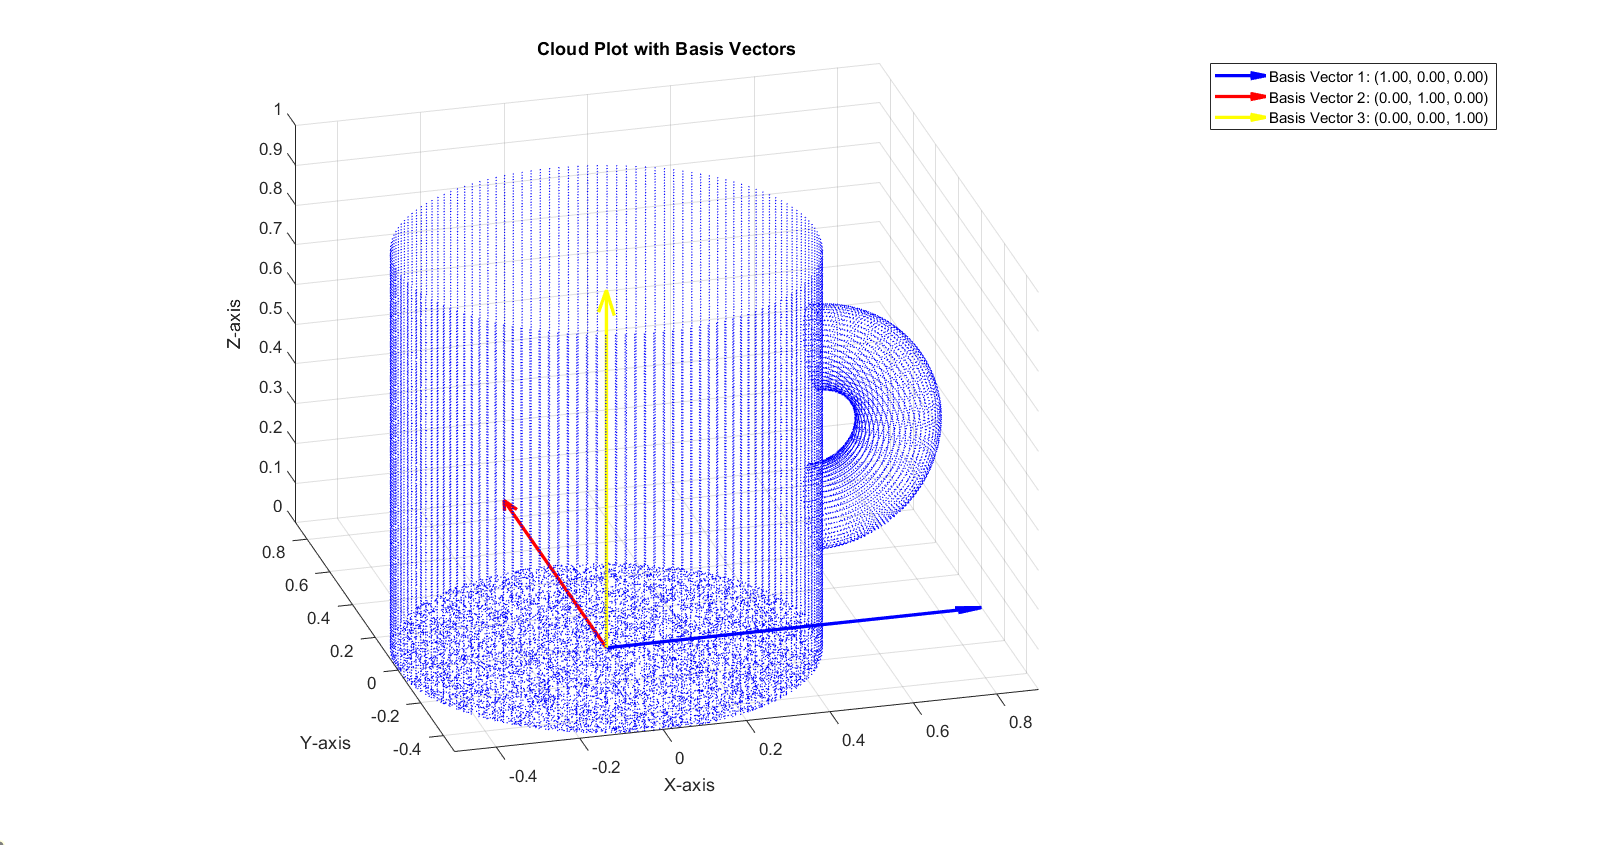
\includegraphics[width=22.62cm, height=11.8cm]{og_mug.png}
\end{center}

\begin{center}
  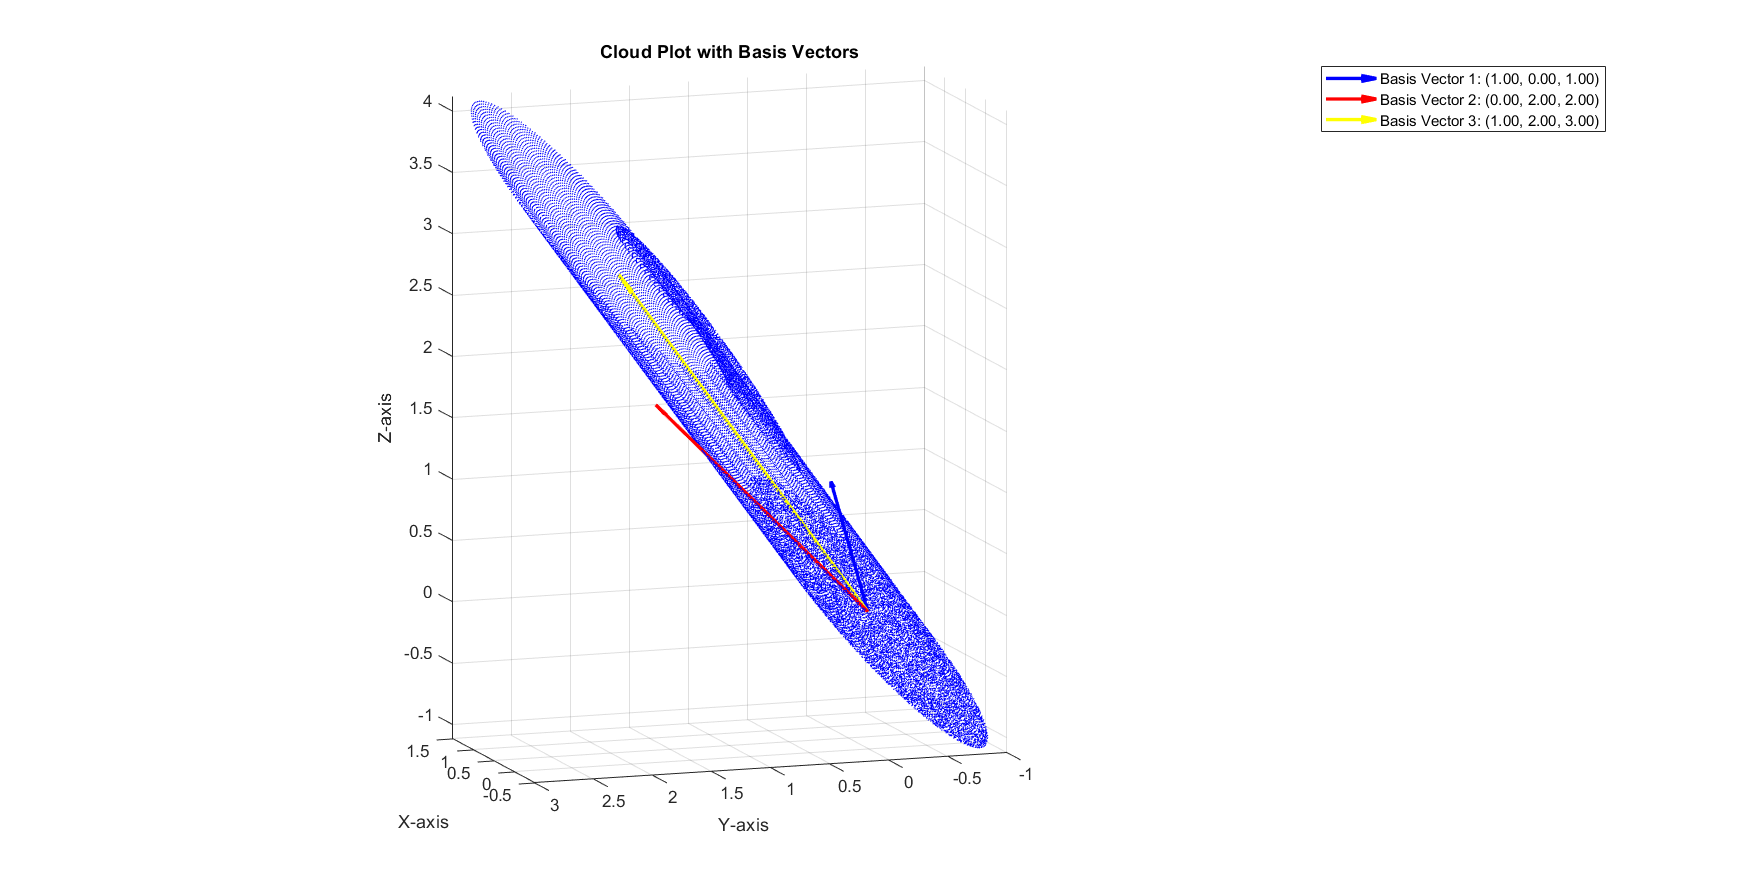
\includegraphics[width=22.62cm, height=11.44cm]{squished_mug.png}
\end{center}

Many matrices have this same effect, where the space to which vectors are sent via transformation differs from the original space of the mapping. 

This phenomenon is very important for the idea of invertibility (and more ideas later in the course), and deals with sets of vectors related to linear transformations called the \emph{image} and \emph{kernel} of a transformation.


First, we define the image of a transformation simply as the set of all mapped-to vectors by a transformation.

Let's discuss some terminology related to linear transformations (and more generally, functions). 

\begin{definition}
  Let $V$ and $W$ be vector spaces and $T$ a linear transformation from vectors in $V$ to vectors in $W$. That is, if $\vec{v}$ is in $V$, then $T(v)$ is in $W$.

  \begin{center}
    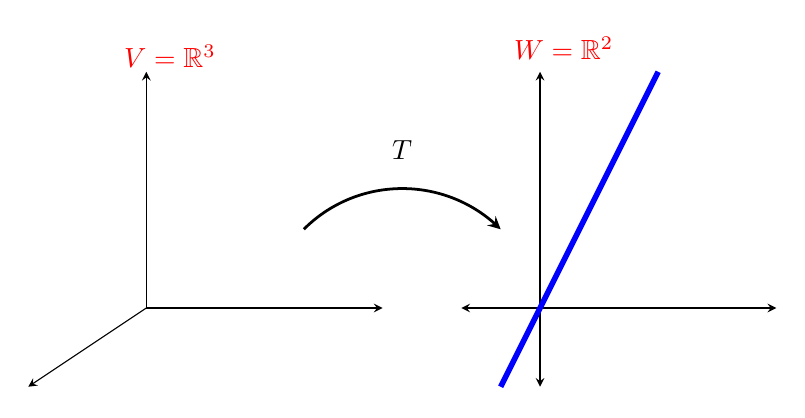
\begin{tikzpicture}[scale=1]
     
      \draw[->] (0,0)--(3,0);
      \draw[->] (0,0)--(0,3);
      \draw[->] (0,0)--(-1.5,-1);
      
      % Labels for the new nodes
      \node[red] at (5.3,3.3) (W) {$W=\RR^2$}; % Near the top of the diagonal axis
      \node[red] at (0.3, 3.2) (V) {$V=\RR^3$}; % Near the top of the vertical axis
       
      \draw[<->] (4,0)--(8,0);
      \draw[<->] (5,-1)--(5,3);
      \draw[line width=2pt,blue](4.5,-1)--(6.5,3);
      \node[] at (3.25, 2)   (b) {$T$};
      \draw [->,line width=1pt,-stealth]  (2,1) to[out=45] (4.5, 1);
     %\node[blue] at (7, 2.3)   (b) {$\mbox{im}(T)$};
     
    \end{tikzpicture}
    \end{center}

  We call $V$ the \emph{domain} of $T$ and $W$ the \emph{codomain} of $T$. In the preceding figure, the map $T$ takes vectors in $\RR^3$ to a line within $\RR^2$. We would say $V$ is $\RR^3$, and $W$ is $\RR^2$.
\end{definition}

Said plainly, the domain of $T$ is the set of vectors that get mapped by $T$, and the codomain of $T$ is all of the mapped-to vectors. 

In the mug example, the set of vectors making the mug picture are in $\RR^3$, so $\RR^3$ is the \wordChoice{\choice[correct]{domain}\choice{co-domain}} of the transformation with matrix $A$. The resulting squished mug plane still lives in $\RR^3$, so the \wordChoice{\choice{domain}\choice[correct]{co-domain}} of $T$ is still $\RR^3$. 

Since the matrix $A=\begin{bmatrix}
  1&0&0\\
  0&1&0\\
\end{bmatrix}$ is a $2x3$ matrix, it takes in vectors in $\RR^3$ and outputs vectors in $\RR^2$, so the \wordChoice{\choice[correct]{domain}\choice{co-domain}} is $\RR^3$ and the \wordChoice{\choice{domain}\choice[correct]{co-domain}} is $\RR^2$.

This distinction could still be more refined, however. For instance we want better language to describe that the result of the mug-squishing matrix $A$ was not just $\RR^3$, but rather a plane within $\RR^3$. Similarly, the transformation $T$ in the preceding figure doesn't map to all of $\RR^2$, but just to a line \emph{within} $\RR^2$. This distinction is important, as we will elaborate. For this, we say that the squished-mug plane and the line from $T$ are the \emph{images} of the transformations.

\begin{definition}\label{def:imageofT}
Let $V$ and $W$ be vector spaces and let $T:V\rightarrow W$ be a linear transformation.  

The \dfn{image} of $T$, denoted by $\mbox{im}(T)$, is the set
$$\mbox{im}(T)=\{T(\vec{v})\text{ in }W\text{ such that }\vec{v}\in V\}$$.

In other words, the image of $T$ consists of all vectors $T(\vec{v})$ that live in the target space $W$.
\end{definition}

\begin{center}
  \youtube{C2D_5GPbQAs}
\end{center}

\begin{remark}
  This reducing of a function's image to a smaller set within the codomain is not unique to linear algebra. Many functions you've encountered thus far have a similar effect. 

  The function $f(x)=x^2$, for instance, only maps to nonnegative real numbers, which is smaller than the codomain set $\RR$.
\begin{center}
  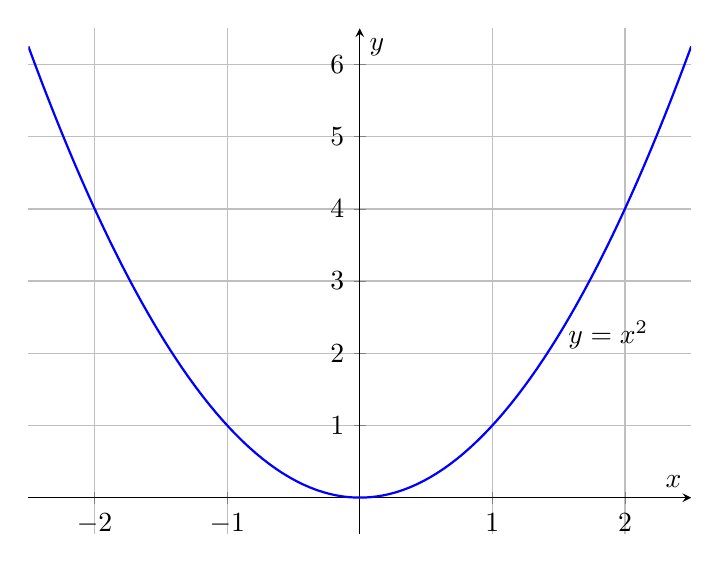
\begin{tikzpicture}
    \begin{axis}[
        axis lines=middle,
        xlabel={$x$},
        ylabel={$y$},
        xmin=-2.5, xmax=2.5,
        ymin=-0.5, ymax=6.5,
        grid=both,
        major grid style={line width=0.5pt, draw=gray!50},
        minor grid style={line width=0.2pt, draw=gray!20},
        width=10cm, height=8cm,
        samples=100,
        domain=-2.5:2.5,
        ]
        \addplot[blue, thick] {x^2};
        \node at (axis cs:1.5,2.25) [anchor=west] {$y=x^2$};
    \end{axis}
\end{tikzpicture}
\end{center}
\end{remark}
 
\begin{example}\label{ex:image1}
Consider the linear transformation $T:\RR^3\rightarrow \RR^2$ with standard matrix
$$A=\begin{bmatrix}1&2&3\\2&4&6\end{bmatrix}$$
 
\begin{enumerate}
\item\label{item:impart1}
Find $\mbox{im}(T)$.
\item\label{item:impart2}
Illustrate the action of $T$ with a sketch.
 
\end{enumerate}
\begin{explanation}
 
\ref{item:impart1} Since the image of $T$ is the set of all possible vectors $T(\vec{v})$ where $\vec{v}$ is a vector in $\RR^3$, let's see what $T$ does to an arbitrary vector $\vec{v}=\begin{bmatrix}a\\b\\c\end{bmatrix}$. Using the matrix $A$, we get 
 
$$T(\vec{v})=A\vec{v}=\begin{bmatrix}1&2&3\\2&4&6\end{bmatrix}\begin{bmatrix}a\\b\\c\end{bmatrix}=a\begin{bmatrix}1\\2\end{bmatrix}+b\begin{bmatrix}2\\4\end{bmatrix}+c\begin{bmatrix}3\\6\end{bmatrix}$$
 
This makes sense because we know that matrix multiplication gives a linear combination of the columns of $A$.  We conclude that
$$\mbox{im}(T)=\mbox{span}\left(\begin{bmatrix}1\\2\end{bmatrix}, \begin{bmatrix}2\\4\end{bmatrix}, \begin{bmatrix}3\\6\end{bmatrix}\right)$$
 
Every column of $A$ is a scalar multiple of $\begin{bmatrix}1\\2\end{bmatrix}$.  Thus,
 
$$\mbox{im}(T)=\mbox{span}\left(\begin{bmatrix}1\\2\end{bmatrix}, \begin{bmatrix}2\\4\end{bmatrix}, \begin{bmatrix}3\\6\end{bmatrix}\right)=\mbox{span}\left(\begin{bmatrix}\answer{1}\\\answer{2}\end{bmatrix}\right)$$
 
The image of $T$ is a line in $\RR^2$ determined by the vector $\begin{bmatrix}\answer{1}\\\answer{2}\end{bmatrix}$.
 
\ref{item:impart2} The following sketch illustrates that $T$ transforms $3$-D space to a line in $2$-D.
 
\begin{center}
\begin{tikzpicture}[scale=1]
 
  \draw[->] (0,0)--(3,0);
  \draw[->] (0,0)--(0,3);
  \draw[->] (0,0)--(-1.5,-1);
 
   
  \draw[<->] (4,0)--(8,0);
  \draw[<->] (5,-1)--(5,3);
  \draw[line width=2pt,blue](4.5,-1)--(6.5,3);
  \node[] at (3.25, 2)   (b) {$T$};
  \draw [->,line width=1pt,-stealth]  (2,1) to[out=45] (4.5, 1);
 \node[blue] at (7, 2.3)   (b) {$\mbox{im}(T)$};
 
\end{tikzpicture}
\end{center}
\end{explanation}
\end{example}
 
 
The key takeaway from Example \ref{ex:image1} is that the image of a linear transformation $T$ with matrix $A$ is the span of the columns of $A$.  Because of how matrix multiplication is defined, this is true for any linear transformation $T:\RR^n\rightarrow \RR^m$.

\begin{theorem}
  The image of a linear transformation $T$ (with associated matrix $A$) from $V$ to $W$ is the span of the columns of $A$.
\end{theorem}

We also need the following important theorem that helps us discern information from the \texttt{rref}. The \emph{why} of the theorem is explained in the video that follows, which also introduces Example \ref{ex:image2}.

\begin{theorem}
  If $A$ is an $m\times n$ matrix and columns $i_1, i_2, \ldots i_k$ are pivot columns of \texttt{rref(A)}, then columns $i_1, i_2, \ldots i_k$ of $A$ are linearly independent vectors in $\RR^n$, and all other columns of $A$ are linearly dependent on columns $i_1, i_2, \ldots i_k$.

  As an example, if $A=\begin{bmatrix}
    1 & 2 & 3\\
    0 & 2 & 2 \\
    1 & 0 & 1
  \end{bmatrix}$, then \texttt{rref(A)}$=\begin{bmatrix}
    1 & 0 & 1\\0&1&1\\0&0&0
  \end{bmatrix}$. Columns $1\&2$ of \texttt{rref(A)} are pivots, so the first two columns of $A$ are linearly independent. The third column of \texttt{rref(A)} is not a pivot, and so the third column of $A$ linearly depends on the first two. 
\end{theorem}

\begin{center}
  \youtube{zWVU588fsAE}
\end{center}
 
\begin{example}\label{ex:image2}
Let $T:\RR^5\rightarrow \RR^4$ be a linear transformation with standard matrix $$A=\begin{bmatrix}1 & 2 & 2 &-1 & 0\\-1 & 3 & 1 & 0 & -1\\3 & 0 & 0 & 3 & 6\\ 1 & -1 & 1 & -2 & -1\end{bmatrix}$$
Find $\mbox{im}(T)$ and $\mbox{dim}(\mbox{im}(T))$.
\begin{explanation}
As in Example \ref{ex:image1}, the image of $T$ is given by
$$\mbox{im}(T)=\mbox{span}\left(\begin{bmatrix}1\\-1\\3\\1\end{bmatrix}, \begin{bmatrix}2\\3\\0\\-1\end{bmatrix}, \begin{bmatrix}2\\1\\0\\1\end{bmatrix}, \begin{bmatrix}-1\\0\\3\\-2\end{bmatrix}, \begin{bmatrix}0\\-1\\6\\-1\end{bmatrix}\right)$$

This time it is harder to detect the vectors that can be eliminated from the spanning set without affecting the span.  We have to rely on the reduced row-echelon form of $A$.
 
$$\begin{bmatrix}1 & 2 & 2 &-1 & 0\\-1 & 3 & 1 & 0 & -1\\3 & 0 & 0 & 3 & 6\\ 1 & -1 & 1 & -2 & -1\end{bmatrix}  \rightsquigarrow \begin{bmatrix} 1 & 0 & 0 & \answer{1} & \answer{2}\\0 & 1 & 0 & \answer{1} & \answer{1}\\0 & 0 & 1 & \answer{-2} & \answer{-2}\\ 0 & 0 & 0 & \answer{0} & \answer{0} \end{bmatrix}$$
 
Because the first three columns are pivot columns, these columns are linearly independent and complete the spanning set.  Therefore,
$$\mbox{im}(T)=\mbox{span}\left(\begin{bmatrix}1\\-1\\3\\1\end{bmatrix}, \begin{bmatrix}2\\3\\0\\-1\end{bmatrix}, \begin{bmatrix}2\\1\\0\\1\end{bmatrix}\right)$$

Because of this, $\mbox{dim}(\mbox{im}(T))=\answer{3}$.
\end{explanation}
\end{example}
 
Tracking the dimension of $\mbox{im}(T)$ is a quick measurement on $T$ that can be useful, particularly for determining properties of $T$, such as invertibility. This constitutes the \emph{rank} of a linear transformation.
 
\begin{definition}\label{def:rankofT}
The \dfn{rank} of a linear transformation $T:V\rightarrow W$, is the dimension of the image of $T$.
$$\mbox{rank}(T)=\mbox{dim}(\mbox{im}(T))$$
\end{definition}

 
\subsection*{The Kernel of a Linear Transformation}

If a linear transformation squishes vectors to form an image of smaller dimension than the codomain (such as occurs in the mug), then some of the vectors in the domain must vanish. The set of vectors that vanish under a transformation $T$ is called the \emph{kernel} of $T$, and can be as explicitly described as the image of $T$.
 
\begin{definition}\label{def:kernel}
Let $V$ and $W$ be vector spaces, and let $T:V\rightarrow W$ be a linear transformation.  The \dfn{kernel} of $T$, denoted by $\mbox{ker}(T)$, is the set
$$\mbox{ker}(T)=\{\vec{v}\text{ in }V\text{ such that }T(\vec{v})=\vec{0}\}$$
In other words, the kernel of $T$ consists of all vectors of $V$ that map to $\vec{0}$ in $W$.
\end{definition}

It is important to pay attention to the locations of the kernel and the image.
 
\begin{center}
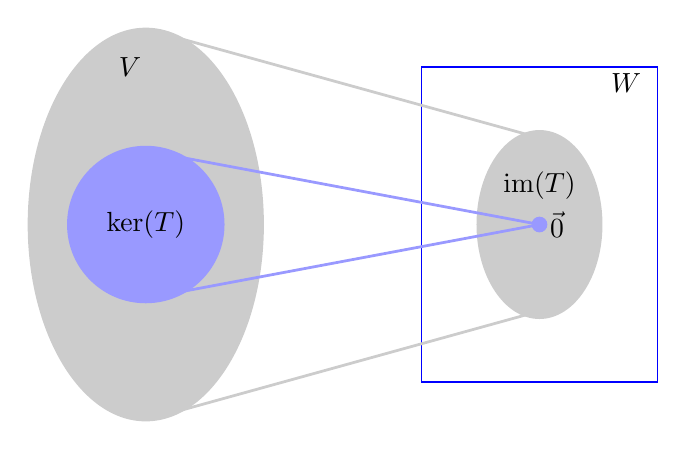
\begin{tikzpicture}
\fill[gray!40] (0,0) ellipse (1.5cm and 2.5cm);
\fill[blue!40!white] (0,0) ellipse (1cm and 1cm)node[black]{$\mbox{ker}(T)$};
 
\draw[blue] (3.5,2) rectangle (6.5,-2);
\node[] at (6.1, 1.8)   (b) {$W$};
\fill[gray!40] (5,0) ellipse (0.8cm and 1.2cm);
\fill[blue!40!white] (5,0) circle (0.1cm);
 
\draw[gray!40,line width=1pt](0.3,2.4)--(5,1.1);
\node[] at (-0.2, 2)   (b) {$V$};
\node[] at (5, 0.5)   (b) {$\mbox{im}(T)$};
\draw[gray!40, line width=1pt](0.3,-2.4)--(5,-1.1);
 
\draw[blue!40!white, line width=1pt](0.2,.9)--(5,0);
\draw[blue!40!white, line width=1pt](0.2,-0.9)--(5,0)node[below, right][black]{$\vec{0}$};
 
\end{tikzpicture}
\end{center}
 
We now focus on describing $\mbox{ker}(T)$ much like we described $\mbox{im}(T)$. Here, we want specifically to determine whether vectors get mapped to $\vec{0}$, which amounts to solving the vector equation $A\vec{v}=\vec{0}$, if $A$ is the matrix associated with $T$.

We again will appeal to the reduced row echelon form of a matrix, and have a similar theorem that relates the reduced row echelon form of a matrix to its kernel as we did with its image. The theorem is motivated in the video that follows.

\begin{theorem}
  If $A$ is an $m\times n$ matrix and columns $j_1, j_2, \ldots j_k$ are \textbf{not} pivot columns of \texttt{rref(A)}, then columns $j_1, j_2, \ldots j_k$ of $A$ span the kernel of $\RR^n$. That is, if $v_{j_1}, v_{j_2}, \ldots, v_{j_k}$ are the associated columns of $A$, and $\vec{w}$ is in $\mbox{span}\left(v_{j_1}, v_{j_2}, \ldots, v_{j_k}\right)$, then $A\vec{w}=\vec{0}$.

  As an example, if $A=\begin{bmatrix}
    1 & 2 & 3\\
    0 & 2 & 2 \\
    1 & 0 & 1
  \end{bmatrix}$, then \texttt{rref(A)}$=\begin{bmatrix}
    1 & 0 & 1\\0&1&1\\0&0&0
  \end{bmatrix}$. The third column of \texttt{rref(A)} is not a pivot, and so any vector of the form $\vec{w}=\lambda \begin{bmatrix}
    3\\2\\1
  \end{bmatrix}$ is in the kernel, meaning $A\vec{w}=0$.
\end{theorem}


\begin{center}
  \youtube{I_E3Jdcv_Kg}
\end{center}
 
\begin{example}\label{ex:kernel} Let $T:\RR^5\rightarrow \RR^4$ be a linear transformation with standard matrix $$A=\begin{bmatrix}1 & 2 & 2 &-1 & 0\\-1 & 3 & 1 & 0 & -1\\3 & 0 & 0 & 3 & 6\\ 1 & -1 & 1 & -2 & -1\end{bmatrix}$$
\begin{enumerate}
\item \label{item:kernelT}
Find $\mbox{ker}(T)$
\end{enumerate}
\begin{explanation}
\ref{item:kernelT} To find the kernel of $T$, we need to find all vectors of $\RR^5$ that map to $\vec{0}$ in $\RR^4$.  This amounts to solving the equation $A\vec{x}=\vec{0}$.
 
Again taking \texttt{rref(A)} yields:
 
$$\mbox{rref}(A)= \begin{bmatrix} 1 & 0 & 0 & 1 & 2\\0 & 1 & 0 & 1 & 1\\0 & 0 & 1 & -2 & -2\\ 0 & 0 & 0 & 0 & 0 \end{bmatrix}$$
 
We have encountered this scenario before when solving systems of equations, particularly when balancing chemical reactions. Since we are solving $A\vec{x}=\vec{0}$, the resulting system of equations has \wordChoice{\choice{two}\choice{three}\choice[correct]{five}} variables, \wordChoice{\choice{two}\choice[correct]{three}\choice{five}} of which are taken by pivots of $rref(A)$, and \wordChoice{\choice[correct]{two}\choice{three}\choice{five}} of which we are free to choose. 

Moreover, because the matrix does not yield any contradictory equations (namely because any non-pivot rows are all $0$s), we can have infinitely many solutions based on the chosen values of the free variables, which we will call $s$ and $t$.

So, $A\vec{x}=\vec{0}$ is satisfied for vectors of the form 

$$\begin{bmatrix}\answer{-1}s\\\answer{-1}s\\\answer{2}s\\s\\\answer{0}s\end{bmatrix},$$

$$\begin{bmatrix}\answer{-2}t\\\answer{-1}t\\\answer{1}t\\\answer{0}t\\t\end{bmatrix},$$

and their linear combinations.

Factoring out $s$ and $t$, we get that all vectors $\vec{x}$ of the form

$$\begin{bmatrix}\answer{-1}\\-1\\\answer{2}\\\answer{1}\\0\end{bmatrix}s+\begin{bmatrix}\answer{-2}\\-1\\2\\0\\\answer{1}\end{bmatrix}t$$

will satisfy $A\vec{x}=\vec{0}$.
 
We conclude that
$$\mbox{ker}(T)=\mbox{span}\left(\begin{bmatrix}\answer{-1}\\-1\\\answer{2}\\\answer{1}\\0\end{bmatrix},\begin{bmatrix}\answer{-2}\\-1\\2\\0\\\answer{1}\end{bmatrix}\right)$$
\end{explanation}

\end{example}

Sometimes we mathematicians can be a little pedantic and as a result we might use two names to describe the same thing in slightly different ways. This will happen from time to time. 

Since technically a linear transformation $T$ isn't always described by a matrix $A$ (in our finite-dimensional examples it is), it behooves us to separately define solutions to the equation $A\vec{x}=\vec{0}$.

\begin{definition}
  The \emph{null space} of a matrix $A$ is the set of all vectors $\vec{x}$ that satisfy the equation $A\vec{x}=\vec{0}$.

  For our purposes, this will always be the same as the kernel of the transformation $T$.
\end{definition}

\begin{example}
  Let's find the image and null space of a transformation $T$ described by the matrix 
  $$B=\begin{bmatrix}
        1 & 3 & 2 & 0 & 0  \\
        0 & 1 & 5 & 2 & 1  \\
        3 & 5 & -14 & -8 &-4  \\
        0 & 0 & 0 & 1 & 1  \\
        \end{bmatrix}$$

  Taking the $\texttt{rref(B)}$ yeilds

  $$\begin{bmatrix}
    \answer{1} & 0 & \answer{-13} & 0 & \answer{3} \\
    0 & \answer{1} & \answer{5} & 0 & \answer{-1} \\
    0 & 0 & 0 & \answer{1} & \answer{1} \\
    0 & 0 & 0 & 0 & 0
  \end{bmatrix}$$

  Despite the ordering of the columns, we have three pivots, in columns $\answer{1}, \answer{2}$ and $\answer{4}$. Thus, the columns of $B$ in these positions are linearly independent and span the image of $T$. Thus,

  $$\mbox{im}(T)=\mbox{span}\left(
  \begin{bmatrix}
  \answer{1} \\
  \answer{0} \\
  \answer{3} \\
  \answer{0}
  \end{bmatrix},
  \begin{bmatrix}
  \answer{3} \\
  \answer{1} \\
  \answer{5} \\
  \answer{0}
  \end{bmatrix},
  \begin{bmatrix}
  \answer{0} \\
  \answer{2} \\
  \answer{-8} \\
  \answer{1}
  \end{bmatrix}
  \right).$$

  This leaves two non-pivot colums from which we have two free variables to generate solutions to $B\vec{x}=\vec{0}$. 

  This yeilds the plane $Null(B)=\text{span}\left( \begin{bmatrix} 
    \answer{13} \\ 
    \answer{-5} \\ 
    \answer{1} \\ 
    \answer{0} \\ 
    \answer{0} 
    \end{bmatrix}, 
    \begin{bmatrix} 
    \answer{-3} \\ 
    \answer{1} \\ 
    \answer{0} \\ 
    \answer{-1} \\ 
    \answer{1} 
    \end{bmatrix}\right)$.
\end{example}

\begin{hint}
Note: Remember that $B$ maps vectors $v$ in $\RR^5$, so there are 5 coordinates in the domain, and you want to correctly assign the right coordinate from the \texttt{rref} information. Moreover, you want to put a 1 in the coordinate associated with the free variable. 
\end{hint}
 

\end{document}